\section{Latency in Cellular Networks}

\subsection{Methodology and Experiement}
\label{sec:methodology}

There are tools for measuring mobile network performance \cite{speedtest, huang2011mobiperf}, but they are generally too specific and can only be applied to limited scope. It's possible to develop a whole suite of measurement tools for mobile contexts, but given the fact that there have been so many tools available \ref{sec:tools}, it would be great to reuse them. One possible approach is to use modem, which will just be another network interface in the computer. Another approach, which can readily use the smartphones that most people have, is by mobile hotspot. The mobile device will serve as first hop, and we can use all the tools on whatever platform the computer is to perform related measurements. Though in most case, people use Bluetooth or Wi-Fi for hotspot, we found that iPhone supports USB tethering. And as we will show in our data analysis part, the latency on the first hop is neglectable. Fig.\,\ref{fig:mobile_networks_method} illustrate the idea of using USB tethering.

\begin{figure}
  \centering
  \includegraphics[width=\linewidth]{../figs/mobile_networks_method.pdf}
  \vspace{-1em}
  \caption{USB tethered computer to perform {\it traceroute} to measure the per-hop latency in cellular backbone.}
  \label{fig:mobile_networks_method}
\end{figure}

For us, we use the system {\it traceroute} to quantify the latency for each hop within cellular networks. The targets for {\it traceroute} are the top 1000 websites we believe most smartphone users will access. Since we are only interested in the cellular backbone networks, after a few initial results, we limit the maximum hop of {\it traceroute} to 13. We've also turned on Autonomous System Number (ASN) lookups for each hop encountered. Fig.\,\ref{fig:traceroute} shows an example trace to Google.

\begin{figure}[!htb]
  \centering
  \includegraphics[width=1.1\linewidth]{../figs/traceroute.pdf}
  \vspace{-1em}
  \caption{Example {\it traceroute} log from an AT\&T iPhone in Berkeley, maximum hop limited to 13, with ASN look-up turned on.}
  \label{fig:traceroute}
\end{figure}


The measurement is conducted between Apr.\,11 to Apr.\,24, when the author isn't in need of his phone. And in total we've collected 191886 measurements, and each includes the timestamp, received signal strength indication (RSSI), radio type (LTE or 4G-LTE), the hop number it belongs to, ASN, hostname, host IP, and the specific delay. It's worth mentioning that the timestamp, RSSI and radio type are the same for each measurement. The reason is due to the difficulty in accessing RSSI and radio type programmatically. The author manually record those data when performing the measurements. Though timestamp can be easily done, we only use it as an indicator of the time when we conduct this measurement. There is no huge need for a finer granularity.

During the experiement, the author paid a trip to San Francisco (SF) through driving, and conducted two measurements for Berkeley-to-SF and SF-to-Berkeley. We will also show the results in the analysis section. 


\subsection{Analysis}
\label{sec:analysis}

We will start by the example trace to Google (Fig.\,\ref{fig:traceroute}). As you can see, the first hop has an IP address $172.20.10.1$, and latencies 0.931 ms, 0.641 ms, 0.640 ms; this is the iPhone used for USB hotstpot. Throughout the experiement, the latency introduced by this USB link is generally small, within 1 ms. Then the second hop reaches out to the first layer 3 router within AT\&T's cellular networks. In LTE architecture, the Evolved Node B (eNode-B) (Fig.\,\ref{fig:mobile_networks_method}) communicates directly with User Equipment (UEs), but it doesn't have layer 3 semantics. It's the access Gateway (AGW) \footnote{AGW also provides termination of the LTE bearer, acts as a mobility anchor point for the user plane. Other key logical functions including MME (Mobility Management Entity) for the Control Plane and SAE PDN GW (System Architecture Evolution Packet Data Network GateWay) for the User Plane \cite{nortel}} that works on IP layer. Afterwards, the packet would goes into AT\&T cellular backbone, traversing routers either with private IP -- 172.16/12 \cite{rekhterrfc}, or with AT\&T's prefix -- 12/8. Interestingly, the ASN reported by {\it traceroute} on the second and third hop is from Amazon's AS (AS16509). This might be due to some incorrect information in the ASN look-up. Then on hop 12, the routes goes out from AT\&T's network to Google's AS.

The same pattern holds for many other traces. And we aggregate them to answer the following question: how is the latency in AT\&T's cellular backbone? Is the latency stable, and are the routes stable? We plot the graph in Fig\,\ref{fig:mobile_latency}. The upper figure shows the latency experienced on each hop (the horizontal axis is hop number, and vertical axis is latency in milliseconds). The red bar is the mean value for each hop, and the blue error bar is 5th and 95th percentile. We've also noted the mean value on top of each bar. The other figure is used to show the routing stability within the cellular networks. We mark different router IP in different color for each hop, and the portion of that color in the bar represents the portion of {\it traceroute} responds from that router for that hop. Keep in mind that the first hop is iPhone through USB tethering. 

From this figure, we found that within the cellular backbone and part of AT\&T's backbone network (from the 2nd hop to 7th hops), the latencies are fairly stable around 40 ms, with variation about 15 ms. The numbers of responding routers are also not many. The second hop has 9 different responders, which are probably all AGWs behind the eNode-B. They doesn't seem to change based on your location (as you can see in Fig\,\ref{fig:mobile_mobile} when we were moving between Berkeley and SF). We conjecture that the fourth hop might be comprised of four load balancer, since anyway the fifth hop is consistent across all the measurements. After first 7 hops, the latency then increases a lot, and the number of routers on each hop also increase drastically. Though the experiement is done for 13 hops, drawing all of them will make the figure less expressive.

Besides the second hop variation across geographical location, from Fig.\,\ref{fig:mobile_mobile}, we can also find that the latencies increase a lot in comparison to Fig.\,\ref{fig:mobile_latency}. This is in part because of the radio access technology change -- in most of the time during the trip, the phone has a connection of 4G-LTE rather than LTE. But the latency on the first hop has also increased a lot, and mobility accounts for part of the degradation. As for the routings inside cellular backbone, again it's fairly stable.

To further understand routing stability, we then take a look at each trace. In a single {\textit traceroute} log, the routing might change, and this rapidly-variable routing is called fluttering in \cite{paxson1997measurements}. For each hop, we see how many different routes the packet has taken, and draw the portion in a stacked bar plot (Fig.\,\ref{fig:mobile_fluttering}). The horizontal axis is still the hop number, the vertical counts the number of different routes in our measured data. For most of the routes within AT\&T cellular backbone, the routes are fairly stable. When approaching the WAN (starting from hop 11), routing fluttering happens more frequent probably because of crossing AS boundries.

\begin{figure}
  \centering
  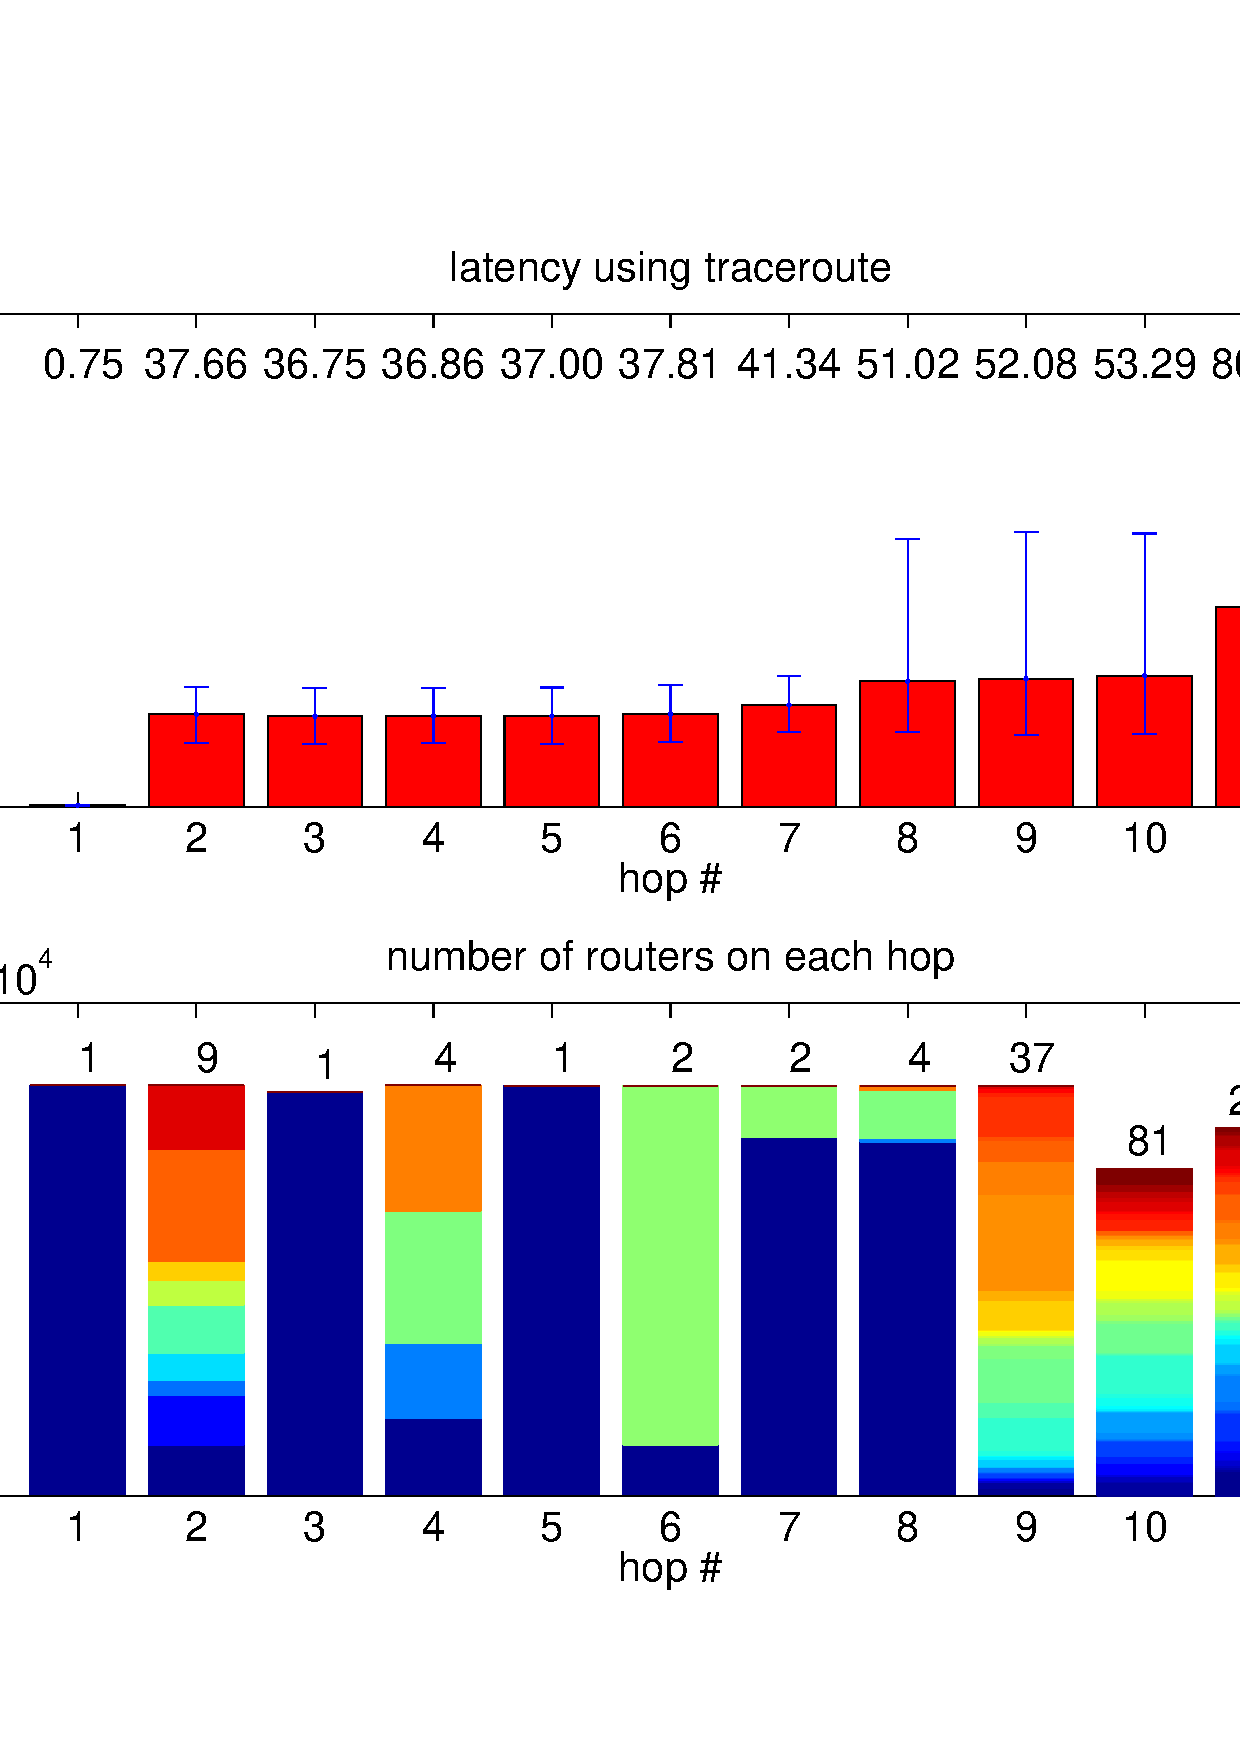
\includegraphics[width=\linewidth]{../figs/mobile_latency.pdf}
  \vspace{-1em}
  \caption{(up) Latency measured in each hop of AT\&T cellular networks; (down) the number of responding routers on each hop}
  \label{fig:mobile_latency}
\end{figure}

\begin{figure}
  \centering
  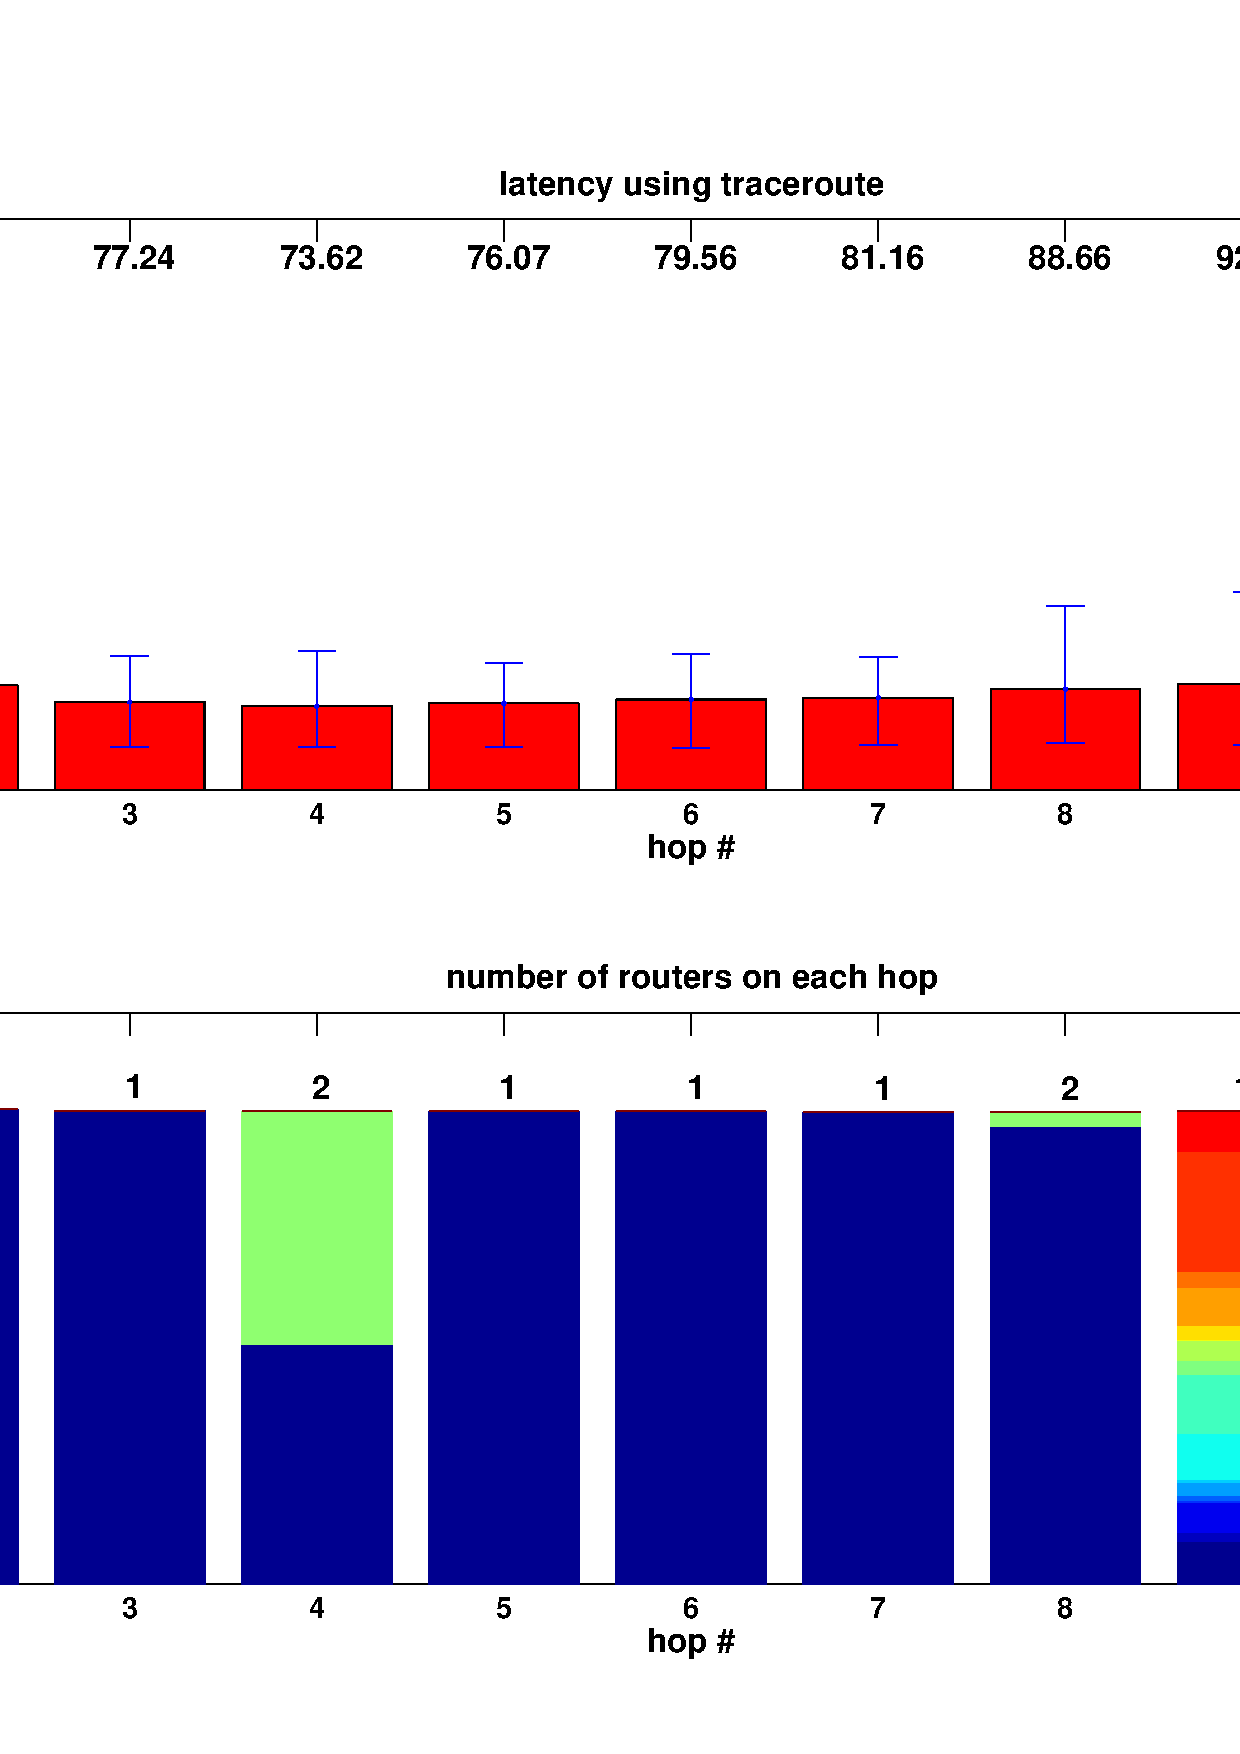
\includegraphics[width=\linewidth]{../figs/mobile_sfo.pdf}
  \vspace{-1em}
  \caption{Measurements conducted when the phone is moving between Berkeley and San Francisco.\\ (up) latency measured in each hop of AT\&T cellular networks; (down) the number of responding routers on each hop}
  \label{fig:mobile_mobile}
\end{figure}

\begin{figure}
  \centering
  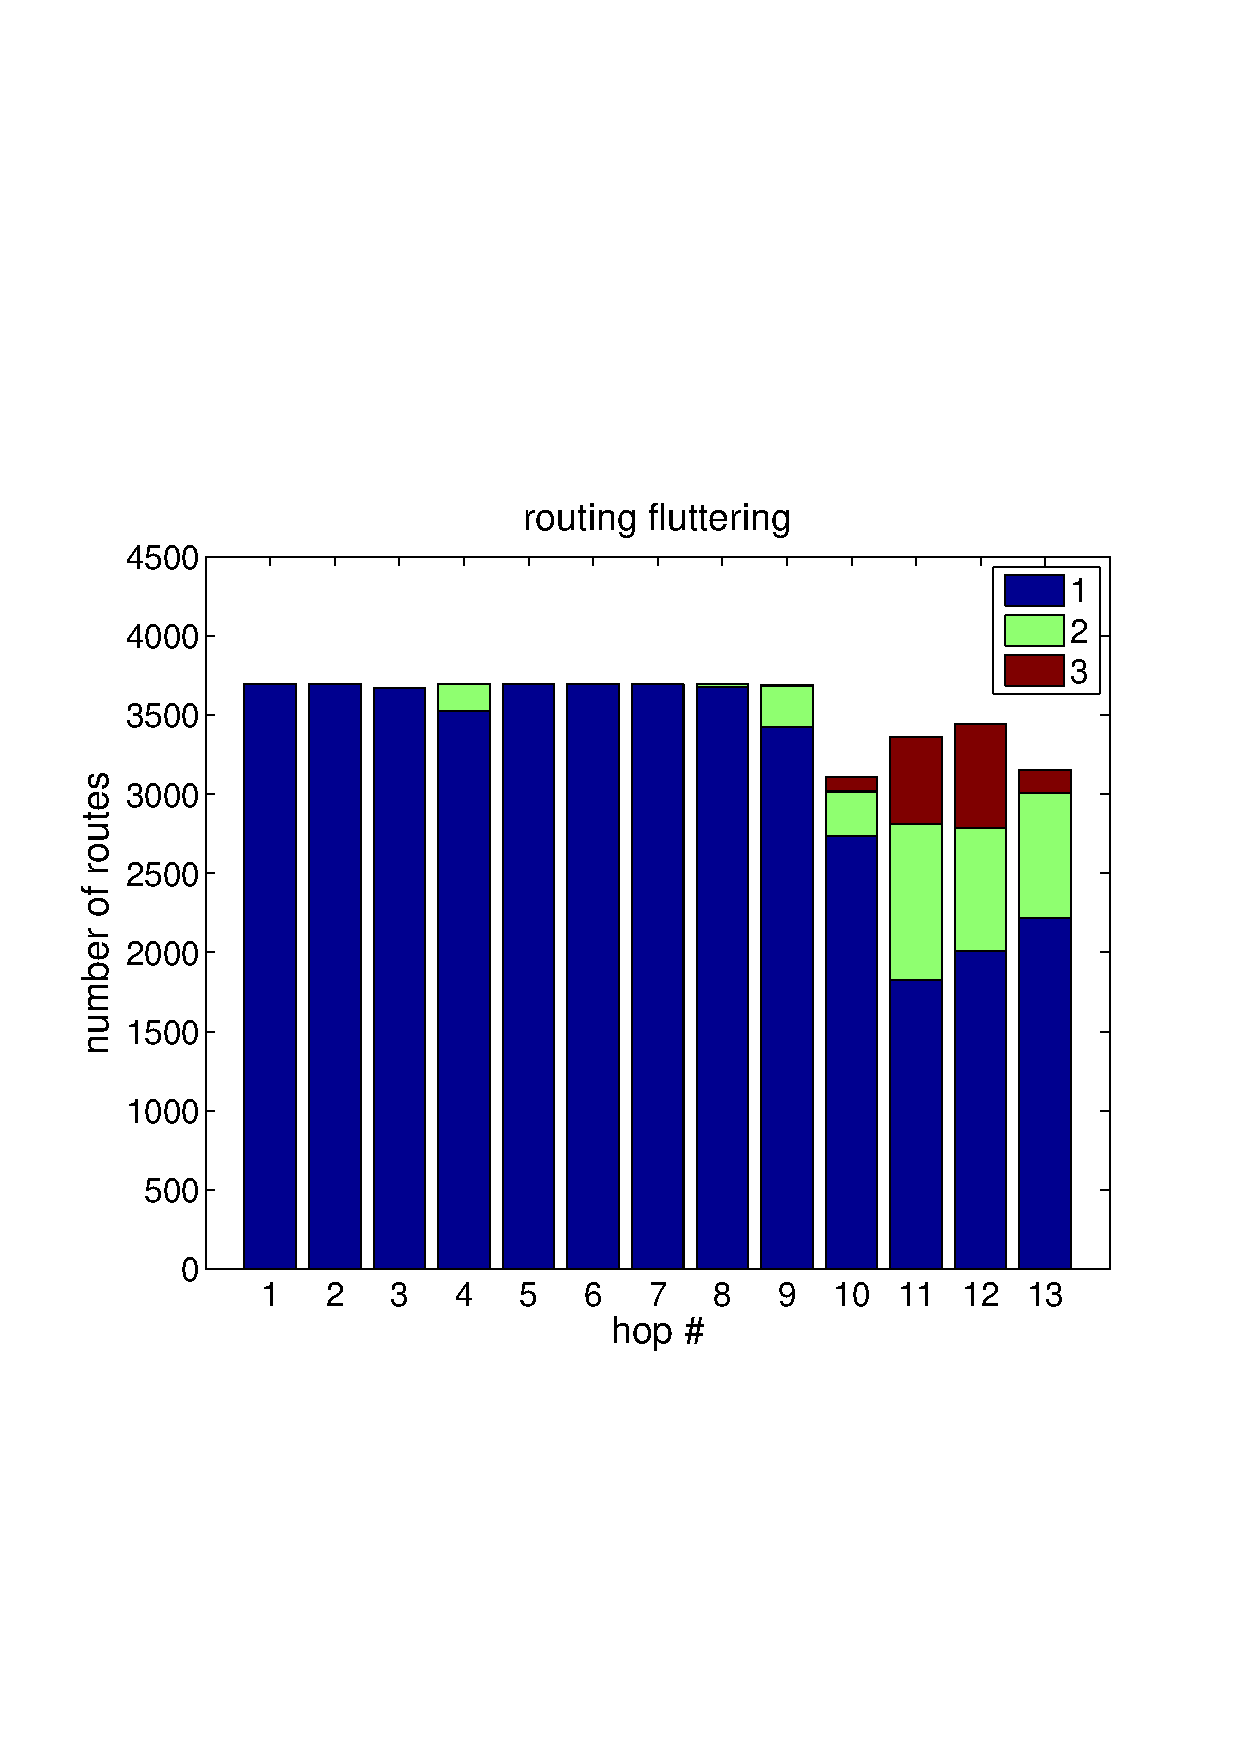
\includegraphics[width=\linewidth]{../figs/mobile_fluttering.pdf}
  \vspace{-1em}
  \caption{Routing fluttering within AT\&T cellular networks}
  \label{fig:mobile_fluttering}
\end{figure}

%%% Local Variables: 
%%% mode: latex
%%% TeX-master: "main"
%%% End: 
